\documentclass[12pt, a4paper]{article}

\usepackage[utf8]{inputenc}
\usepackage[ngerman]{babel}
\usepackage{amsmath, amssymb}
\usepackage[left=2.5cm, right=2.5cm, top=2.5cm, bottom=2.5cm]{geometry}
\usepackage{graphicx}
\usepackage{fancyhdr}
\usepackage{titling}
\usepackage{caption}
\usepackage{subcaption}
\usepackage{setspace}
\usepackage{footmisc}
\usepackage[font=footnotesize,labelfont=bf]{caption}
\usepackage[format=plain, indention=2em]{caption}
\graphicspath{{Image Sources/}}

\newcommand{\subtitle}[1]{%
	\posttitle{%
		\par\end{center}
	\begin{center}\large#1\end{center}
	\vskip0.5em}%
	}
	
\addto\captionsngerman{\renewcommand{\figurename}{Fig.}}
\onehalfspacing
\renewcommand{\subsectionmark}[1]{}
\renewcommand{\footnotelayout}{\setstretch{1.0}\footnotesize}
\renewcommand{\labelenumi}{\Roman{enumi}}
\renewcommand{\labelenumii}{\Roman{enumi}.\roman{enumii}}
\renewcommand{\labelenumiii}{\Roman{enumi}.\roman{enumii}.\roman{enumiii}}
\renewcommand{\labelenumiv}{\Roman{enumi}.\roman{enumii}.\roman{enumiii}.\roman{enumiv}}



\title{Probekapitel W-Seminararbeit}
\subtitle{Funktionsweise der X-Hall Architektur}
\author{Armin Binder }
\date{Juni 2025}

\begin{document}
	\pagestyle{fancy}
	\fancyhf{} 
	\fancyfoot[C]{\thepage}
	
	%\pagenumbering{arabic}
%	\fancyhf{}
%	\fancyfoot[R]{\thepage}
	\maketitle
	\thispagestyle{empty}
	\pagebreak
	
	\tableofcontents
	\thispagestyle{empty}
	\pagebreak
	{
	\section{Vorläufige Gliederung}
	\begin{enumerate}
		\item Abstract
		\item Einführung in Arbeit und Thematik
		\item Funktionsweise der X-Hall-Architektur (Probekapitel)
		\begin{enumerate}
			\item Geschichte und Konzept
			\item Aufbau und Funktionsweise
			\item Vorteile und Nachteile der Architektur
		\end{enumerate}
		\item Design des Sensors
		\begin{enumerate}
			\item Genereller Aufbau des Sensors
			\item Genereller Aufbau der Sensorsonde
			%\item Aufbau des Verstärkers
			%\item Einführung von digitaler Datenverarbeitung und Schnittstelle
			%\item Integration des Sensors mit Handy
		\end{enumerate}
		\item Charakteristika und Validierung des Sensors
		\item Vergleich mit anderen Sensortypen
		\item Fazit
	\end{enumerate}\paragraph{}
	\centering
	Diese Gliederung ist nur von vorläufiger Natur. Änderung der Titel spezifische Punkte und das hinzufügen beziehungsweise entfernen einiger Unterpunkte im Laufe der Finalisierung der Arbeit ist nicht ausgeschlossen.
	\newpage}
	
	\section{Funktionsweise der X-Hall Architektur}
		Im vorherigen Kapitel wurden bereits die grundlegende Funktionsweise von Hall-Sensoren sowie typische Architekturen solcher Systeme behandelt.\paragraph{}
		Die für diese Arbeit gewählte Architektur, die sogenannte \textbf{X-Hall-Architektur} unterscheidet sich aber von den zuvor genannten Architekturen in mehreren relevanten Aspekten. Im Folgenden soll diese spezifische Architektur vorgestellt werden und auf ihre Vor- sowie Nachteile eingegangen werden, ebenso wie auf die Gründe zur Wahl genau dieser %genauen 
		Architektur für diese Arbeit.
		
		\subsection{Geschichte und Konzept}
		Bei der X-Hall-Architektur handelt es sich um eine recht neue Form des Hall-Sensors. Erstmalig wurde sie gegen Ende des Jahres 2018 auf dem IMEKO\footnote{International Measurement Confederation} 
		World Congress vorgestellt \textbf{\cite{cres19}}. \newline
		Die Entwicklung dieser neuen Art Hall-Sensor wurde insbesondere durch den Bedarf für Magnetfeldsensoren mit immer größeren Frequenzbandbreiten vorangetrieben, die grundlegende Bestandteile unter anderem von Sicherheitsschaltungen vieler moderner Stromversorgungskreisläufe sind\textbf{\cite{cres18}\cite{cres19}\cite{cres20}\cite{cres21}}. Die bisher genutzten Sensortypen und Architekturen, wohlgemerkt nicht exklusiv Hall-Sensoren, wiesen aber bereits durch ihren Aufbau alle gewisse Einschränkungen und Probleme auf, die ihre Einsetzbarkeit limitierten\textbf{\cite{cres18}\cite{cres19}\cite{cres21}}. \newline
		Ziel der neuen Sensorarchitektur sollte es also sein, alle Aspekte, die für so einen Magnetfeldsensor relevant sind, in sich zu vereinen\textbf{\cite{cres19}}: 
		\begin{itemize}
			\item Sehr hohe bemessbare Frequenzbandbreiten von Magnetfeldern %Nochmal seperat bestätigen
			\item Fähigkeiten, Gleichspannung (indirekt) zu messen
			\item Mögliche CMOS\footnote{Complementary Metal-Oxide Semiconductor = komplementärer Metalloxid-Halbleiter}-Integration
			\item Galvanische Isolation\footnote{Elektrische funktionale Sektionen sind so voneinander isoliert, dass es keinen direkten Stromfluss zwischen ihnen gibt}
			\item Keine Wärmeabstrahlung
			\item Geringer Flächenbedarf %Kleines Profil
			\item Geringe Produktionskosten
		\end{itemize} \newpage
		Ergebnis dieses Forschungsprojekts war die X-Hall-Architektur.\newline
		Einfach gesagt handelt es sich hierbei um eine Hall-Sonde mit jeweils vier Vorspannungs\footnote{Strom der durch den Sensor fließt, um den Hall-Effekt erst zu ermöglichen}- und vier Auslesekontakten (was jeweils das doppelte der jeweiligen Kontaktarten bei typischen Hall-Sensoren ist), die an der aktiven Fläche des Sensors angebracht sind. Durch eine elektrische Verbindung jeweils zweier diagonal gegenüberliegender Auslesekontakte vor dem eigentlichen Auslesevorgang wird gewährleistet, dass mögliche Defekte und Offsetspannungen\footnote{Ungewollte Spannungen, die selbst dann gemessen werden können, wenn der theoretische Messwert 0 sein sollte} auf der größeren aktiven Fläche unter anderem durch so entstehende Mittelungseffekte kompensiert werden. Dies führt zu einer einer höheren Genauigkeit und Stabilität der Messwerte.
		
		\subsection{Aufbau und Funktionsweise}
		Bei der aktiven Fläche eines X-Hall-Sensors handelt es sich in der Regel um einen oktagonal geformten, sogenannten n-Well\footnote{n-dotierte ``Halbleitertasche'' innerhalb eines p-dotierten Substrats} \cite{cres18}. \newline
		Die n-Dotierung der aktiven Sensorfläche wird aufgrund einer höheren strombezogenen Empfindlichkeit\footnote{Begründet durch höhere Elektronenmobilität in n-Typ-Halbleitern} im Gegensatz zu p-dotierten Halbleitern präferiert. %bevorzugt?
		Auch ist die Umschließung des n-Wells mit einem p-dotierten Material zwar für die grundlegende Sensorfunktion nicht essenziell, %auf nichtverwendung in Arbeit aufgrund komplexität hinweisen? 
		sollte jedoch  angestrebt werden, da nur so eine effektive elektrische Isolation gegenüber dem Substrat erreicht werden kann\cite{cres20}.\newline
		Der Zugang zur aktiven Fläche erfolgt über insgesamt acht Kontakte, die sich in vier großflächige Vorspannungskontakte und vier möglichst kleine Auslesekontakte unterteilen lassen. Die Vorspannungskontakte profitieren aufgrund ihrer Größe von sehr niedrigen Widerständen beim Anlegen der Vorspannung, während die Auslesekontakte so klein wie möglich sein sollten, da so die möglichen Effekte parasitärer Kapazitäten\footnote{Unerwünschte Kapazität, die durch geringe physische Nähe zwischen elektrischen Bauteilen entsteht} % , ???
		wie etwa Signalverzerrungen oder erhöhtes Rauschen des Signals minimiert werden können\cite{cres19}.\newline
		An die in Fig.~\ref{fig:1}(a) als B und T bezeichneten Vorspannungskontakte werden nominal gleiche Vorspannungsströme ($I_A=I_B$) angelegt, während die als L und R bezeichneten Kontakte jeweils als Erdungskontakte dienen\cite{cres19}. Die Auslesekontakte sind von 1 bis 4 durchnummeriert.\newline
		In der aktuellen Konfiguration kann die gesamte Sensorsonde in zwei innere Sensorsonden untergliedert werden, die in Fig.~\ref{fig:1}(a) als Probe A und Probe B bezeichnet sind. Dies ist eine direkte Folge aus der in Fig.~\ref{fig:1}(b) gezeigten Stromstärkeverteilung zwischen den Kontakten auf dem Halbleiter, da der Strom über die Erdung bereits abgeführt wird, bevor er die zweite innere Sonde erreichen kann\cite{cres20}.
		\begin{figure}
			\centering
				%Fig. 1-a
				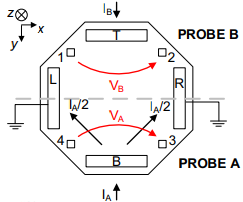
\includegraphics[height=5cm]{Fig1.1}	
				\hspace{0.5cm}
				%Fig. 1-b
				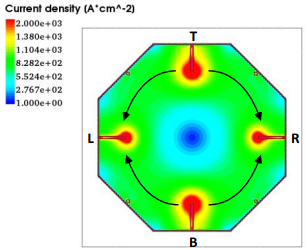
\includegraphics[height=5cm]{Fig1.2}
				\caption{(a) Skizze des Aufbaus der X-Hall-Sonde, (b) Stromstärkeverteilung auf der X-Hall-Sonde, basierend auf einer beispielhaften Vorstromstärke von $I_A=I_B=500\mu{A}$}
				\label{fig:1}
		\end{figure}\newline
		Diese inneren Sonden funktionieren, unabhängig voneinander, jeweils wie gewöhnliche stromverzweigende Hall-Sonden, bei denen die jeweilige Stromdichte $J_A$ oder $J_B$ in zwei gleiche Stromdichten $J_{A,L}$ und $J_{A,R}$ beziehungsweise $J_{B,L}$ und $J_{B,R}$ aufgespalten werden. Dementsprechend gilt für jeweiligen Potentiale zwischen den Messkontakten 1 und 2 beziehungsweise 3 und 4 in Abwesenheit eines Magnetfelds: $V_A=V_B=0$ \cite{cres21}.\newline
		Liegt nun ein Magnetfeld $B_Z$ vor, entsteht aufgrund der Lorentzkräfte die auf die Ladungsträger wirken ein Ungleichgewicht im Stromfluss, was dazu führt, dass nun vereinfacht $V_A=V_\mathrm{Hall}$ und $V_B=-V_\mathrm{Hall}$ (Da der Stromfluss in der zweiten inneren Sonde in die entgegengesetzte Richtung des Stroms von Sonde A verläuft).\newline
		In Realität lassen sich jedoch Asymmetrien in der Sensorstruktur, globale Inhomogenitäten von Materialien und andere Defekte nicht vermeiden, weshalb für die gemessenen Spannungen $V_A$ und $V_B$ tatsächlich gilt:
		\begin{equation}
			V_A=V_\mathrm{H,Sonde}+V_\mathrm{OS}^{(A)}
			\label{eq:1}
		\end{equation}
		\begin{equation}
			V_B=-V_\mathrm{H,Sonde}+V_\mathrm{OS}^{(B)}
			\label{eq:2}
		\end{equation}
		$V_\mathrm{OS}^{(A)}$ und $V_\mathrm{OS}^{(B)}$ sind die Offsetspannungen der jeweiligen inneren Sonde\cite{cres20}.\newline
		Da beide inneren Sonden sich nichtsdestotrotz die gleiche aktive Sensorfläche teilen, kann angenommen werden, dass das Vorzeichen von $V_\mathrm{OS}^{(A)}$ und $V_\mathrm{OS}^{(B)}$ identisch ist, auch wenn sich ihre jeweiligen Werte aufgrund lokaler Defekte unterscheiden können\cite{cres21}. Deshalb kann angenommen werden, dass die Hauptquelle der Offsets sehr wahrscheinlich für beide inneren Sonden die selbe ist\cite{cres20}.\newline
		\begin{figure}
			\centering
			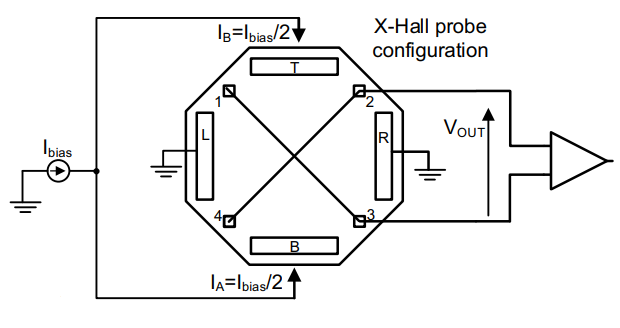
\includegraphics[height=5cm]{Fig2}
			\caption{Schematischer Schaltplan einer X-Hall-Sonde}
			\label{fig:2}
		\end{figure}
		Wie in Fig.~\ref{fig:2} gezeigt besteht die eigentliche und namensgebende Besonderheit der X-Hall-Architektur in einer Überkreuzverbindung der diagonal gegenüberliegenden Paare von Auslesekontakte (1 mit 3 und 2 mit 4). Daraus folgt:
		\begin{equation}
			V_A=-V_B=V_\mathrm{H,Sonde}
			\label{eq:3}
		\end{equation}
		Unter der Annahme gleicher Vorzeichen beider Offsetspannungen und einer Substitution von (\ref{eq:1}) und (\ref{eq:2}) in (\ref{eq:3}) wird  impliziert:
		\begin{equation}
			V_\mathrm{OS}^{(A)}=V_\mathrm{OS}^{(B)}=0
			\label{eq:4}
		\end{equation}
		Physikalisch gesehen erzeugt die Überkreuzverbindung der Auslesekontakte eine  Randbedingung in der aktiven Fläche, welche die Ladungsverteilung so beeinflusst, dass Offsetspannungen minimiert werden \cite{cres21}. 
		Durch die Überkreuzverbindung sind beide Kontakte elektrisch verbunden, was dazu führt, dass sich die Ströme der beiden Kontakte gegenseitig ausbalancieren. %Dies ist Teil der typischen Ladungsverteilung hin zum energetisch günstigsten Zustand des Systems. 
		Aufgrund dieser ladungsverschiebenden Effekte gleicht das System selbstständig ungewollte Offsets oder Defekte und damit verbundene energetisch ungünstige Ladungsverteilungen – ob lokal oder global – aus. %da das System bestrebt ist, seinen energetisch günstigen Zustand zu erreichen. 
		So werden Anteile dieser ungünstigen Ladungsverteilungen in den tatsächlich ausgelesenen Messwerten minimiert.\newline
		Trotzdem wird es immer vereinzelte lokale Defekte und Offsets geben, die zu einer verbleibenden Offsetspannung führen und jeweils zu $V_A$ und $V_B$ hinzugerechnet werden müssen. Die X-Hall-Architektur strebt also primär an, globale Defekte und Offsets mit starkem Einfluss auf Messergebnisse auszugleichen und nicht, diese vollständig zu eliminieren\cite{cres21}.
		
		\subsection{Vorteile und Nachteile der Architektur}
			\centering
		Dieser Abschnitt wird in der vollständigen Arbeit weiter ausgeführt werden (Inhalt: Vor- und Nachteile der Architektur und evtl. eingehen auf diese als Gründe für die Wahl dieser spezifischen Sensorarchitektur)
		
		
		
		
		
		%\clearpage
		\newpage
		\begin{thebibliography}{}
			\addcontentsline{toc}{section}{Literaturverzeichnis}
			\bibitem{cres18}
			\textbf{M. Crescenti et. al.}, Bandwith enhancement in Hall Probe by X-Hall DC biasing. XXII World Congress of International Measurement Confederation (IMEKO 2018), Journal of Physics: Conf. Series \textbf{1065} (2018) 052031, Belfast, United Kingdom, 2018, doi: 10.1088/1742-6596/1065/5/052031
			
			\bibitem{cres19}
			\textbf{M. Crescenti et. al.}, A  Broadband Current Sensor based on the X-Hall Architecture. 2019 26th IEEE International Congerence on Electronics, Circuits and Systems (ICECS), Genoa, Italy, 2019, pp. 807-810, doi: 10.1109/ICECS46596.2019.8964955
			
			\bibitem{cres20}
			\textbf{M. Crescenti et. al.}, Experimental Assessment of a Broadband Current Sensor based on the X-Hall Architecture. 2020 IEEE International Instrumentation and Measurement Technology Conference (I2MTC), Dubrovnik, Croatia, 2020, pp. 1-6, doi: 10.1109/I2MTC43012.2020.9128994
						
			\bibitem{cres21}
			\textbf{M. Crescenti et. al.}, The X-Hall Sensor: Towards Integrated Broadband Current Sensing. IEEE TRANSACTIONS ON INSTRUMENTATION AND MEASUREMENT, vol. 70, pp. 1-12, 2021, doi: 10.1109/TIM.2020.3036764
			
			\bibitem{paun13}
			\textbf{Maria-Alexandra Paun, JM. Salesse, M. Kayal}, Hall Effect Sensors Design, Integration and Behavior Analysis. Journal of Sensors and Actuator Networks, 2013, 2, pp. 85-97, doi: 10.3390/jsan2010085
			
			\bibitem{singh19}
			\textbf{Navinder Singh, Arun M. Jayannavar}, A Brief history of mangnetism. Physical Research Laboratory Ahmedabad and IOP Bhubaneswar, India, 2019, arXiv:1903.07031v1 [physics.pop-ph]
			
			\bibitem{metioui22}
			\textbf{Abdeljalil Métioui}, Brief Historical Review about
			Magnetism: From the Ancient Greeks up the Beginning of the XXth Century. Journal of Biomedical Research and Environmental Sciences (J Biomed Res Environ Sci), doi: 10.37871/jbres1561
			
			
			
		\end{thebibliography}
		
		\section*{Grafikquellen}
		\addcontentsline{toc}{section}{Grafikquellen}
		\begin{description}
			\item \textbf{Fig. 1-a}: Übernommen aus \cite{cres18}, Fig. 1a
			\item \textbf{Fig. 1-b}: Übernommen aus \cite{cres20}, Fig. 2
			\item \textbf{Fig. 2}: Übernommen aus \cite{cres18}, Fig. 2a
		\end{description}
		
		
\end{document}
